%%%%%%%%%%%%%%%%%%%%%%%%%%%%%%%%%%%%%%%%%%%%%%%%%%%%%%%%%%%%%%%%%%%%%%
%%%%%%%%%%%%%%%%%%%%%%%%%%%%%%%%%%%%%%%%%%%%%%%%%%%%%%%%%%%%%%%%%%%%%%
%%%%%%%%%%%%%%%%%%%%%%%%%%%%%%%%%%%%%%%%%%%%%%%%%%%%%%%%%%%%%%%%%%%%%%
\newpage
\section{Derivatives of Matrix Elements}

For Casimir computations we need derivatives of matrix elements
with respect to rigid displacements and rotations of basis functions.

\subsection{Derivatives by Spherical-Multipole Method}

\subsection{Derivatives by Panel-Panel Integral Method}

We write the panel-panel decomposition of the RWG inner products,
equation (\ref{PPIs}), in the form
%====================================================================%
\begin{subequations}
\begin{align}
 \Big\langle \vb f_a \Big| \vb G(k) \Big | \vb f_b \Big \rangle
&= l_a l_b \sum_{\sigma, \tau=-}^+
   \sigma \tau
   \left\{ H_\bullet(\pan_a^\sigma, \pan_b^\sigma, \vb R) 
           -\frac{1}{k^2} H_\nabla(\pan_a^\sigma, \pan_b^\sigma, \vb R) 
   \right\}
\\
 \Big\langle \vb f_a \Big| \vb C(k) \Big | \vb f_b \Big \rangle
&= 
   \frac{l_a l_b }{ik}
   \sum_{\sigma, \tau=-}^+
   \sigma \tau \cdot 
   H_\times(\pan_a^\sigma, \pan_b^\sigma, \vb R) 
\end{align}
\end{subequations}
%====================================================================%
where
%====================================================================%
\begin{subequations}
\begin{align}
 H_\bullet(\pan_a, \pan_b, \vb R) 
   &=\frac{1}{4A_a A_b} 
     \int_{\pan_a} d\vb y_a \, \int_{\pan_b} d\vb y_b \,
     h_\bullet(\vb y_a, \vb y_b)
     \phi\big(k, \vb R + \vb y_{a} - \vb y_{b} \big) 
\\
 H_\nabla(\pan_a, \pan_b, \vb R) 
   &=\frac{1}{4A_a A_b} 
     \int_{\pan_a} d\vb y_a \, \int_{\pan_b} d\vb y_b \,
     h_\nabla(\vb y_a, \vb y_b)
     \phi\big(k, \vb R + \vb y_{a} - \vb y_{b} \big) 
\\
 H_\times(\pan_a, \pan_b, \vb R)
   &=\frac{1}{4A_a A_b}
     \int_{\pan_a} d\vb y_a \, \int_{\pan_b} d\vb y_b \,
     h_\times(\vb y_a, \vb y_b, \vb R)
     \psi\big(k, \vb R + \vb y_{a} - \vb y_{b} \big). 
\end{align}
\label{ThreeHFunctions}
\end{subequations}
%====================================================================%
Here we have rewritten the integrals over $\vb x_a, \vb x_b$ in 
equation (\ref{PanelPanelIntegrals}) using new integration variables
defined relative to the panel centroids (Figure \ref{RabFigure}):
%====================================================================%
\numeq{Rab}
{
  \vb x_a=\vb x_{a0} + \vb y_a, 
   \qquad 
   \vb x_b=\vb x_{b0} + \vb y_b, 
   \qquad
   \vb R_{ab} \equiv \vb R = \vb x_{a0} - \vb x_{b0}.
}
%====================================================================%
%####################################################################%
\begin{figure}
\begin{center}
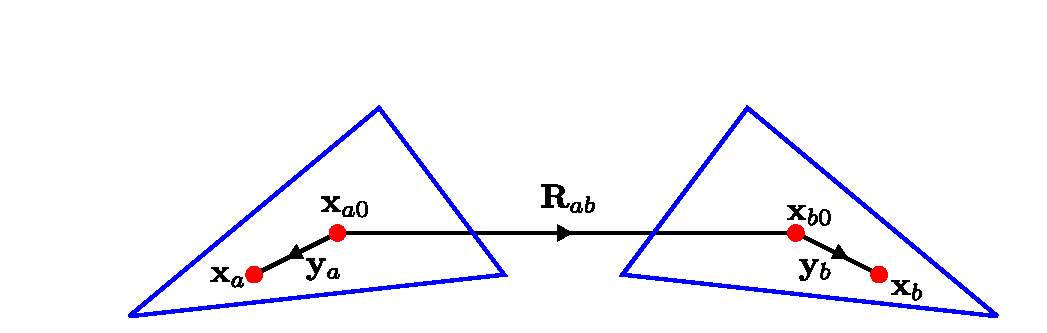
\includegraphics{figures/PPIDerivatives.pdf}
\caption{Notation for equation \ref{Rab}.}
\label{RabFigure}
\end{center}
\end{figure}
%####################################################################%
(In equation (\ref{ThreeHFunctions}), note that $h_\times$, 
unlike $h_\bullet$ and $h_\nabla$, depends on $\vb R$ in 
addition to $\vb y_a, \vb y_b$.)

Now we can take derivatives with respect to the components 
of $\vb R$. Putting $\vb r = \vb R + \vb y_a - \vb y_b)$, we have
\begin{align*}
  \pard{H_\bullet}{\vb R_i}
&= \int d\vb y_a \, \int d\vb y_b \,
   \vb r_i 
   h_\bullet(\vb y_a, \vb y_b)
   \psi\big(k, \vb R + \vb y_a - \vb y_b \big) 
\\
  \pard{H_\nabla}{\vb R_i}
&= \int d\vb y_a \, \int d\vb y_b \,
   \vb r_i 
   h_\nabla(\vb y_a, \vb y_b)
   \psi\big(k, \vb R + \vb y_a - \vb y_b \big)
\\
  \pard{H_\times}{\vb R_i}
&= 
   \int d\vb y_a \, \int d\vb y_b \,
   \vb r_i
   h_\times(\vb y_a, \vb y_b, \vb R)
   \zeta\big(k, \vb R + \vb y_a - \vb y_b \big)
\\
&\qquad + 
   \int d\vb y_a \, \int d\vb y_b \,
   \pard{h_\times(\vb y_a, \vb y_b, \vb R)}{\vb R_i}
   \psi\big(k, \vb R + \vb y_a - \vb y_b \big)
\end{align*}
In the last line, we put
$$ \zeta(k, r) = \Big[ (ikr)^2 -3ikr + 3\Big]\frac{e^{ikr}}{4\pi r^5}$$
[which is defined such that $\nabla \psi(k,|\vb r|) = \vb r \zeta(k, |\vb r|)$]
and we have 
\begin{align*}
 \pard{ h_\times(\vb y_a, \vb y_b, \vb R)}{\vb R_i}
&=\pard{}{\vb R_i} 
   \bigg\{ \Big[ (\vb y_a - \vb Q_a) \times (\vb y_b - \vb Q_b) \Big]
           \cdot \vb R 
   \bigg\}
\\
&= \Big[ (\vb y_a - \vb Q_a) \times (\vb y_b - \vb Q_b) \Big]_i.
\end{align*}

\subsubsection*{Desingularization}

%====================================================================%
\begin{align*}
  \pard{H_\bullet}{\vb R_i}
&= \iint \vb r_i \vb h_\bullet \psi
\\
&= \iint \vb r_i h_{\bullet} \psi\supt{DS}
   +\sum_{n=0}^4 \frac{(ik)^n}{4\pi} B_n 
    \iint \vb r_i h_{\bullet} r^{n-3}
\\[10pt]
%--------------------------------------------------------------------%
  \pard{H_\nabla}{\vb R_i}
&= \iint \vb r_i h_\nabla \psi  
\\
&= \left[ \iint \vb r_i h_{\nabla} \psi\supt{DS}
                 +\sum_{n=0}^4 \frac{(ik)^n}{4\pi} B_n 
                  \iint \vb r_i h_{\nabla } r^{n-3}
           \right]
\\[10pt]
%--------------------------------------------------------------------%
  \pard{H_\times}{\vb R_i}
&=   \iint \vb r_i h_\times \zeta
   + \iint \left( \pard{h_\times}{\vb R_i}\right) \psi
\\
%--------------------------------------------------------------------%
&= \iint \vb r_i h_{\times} \zeta\supt{DS}
    +\iint \left(\pard{h_\times}{\vb R_i}\right)\psi\supt{DS}   
\\ 
&\qquad
   +\left[ \sum_{n=0}^5 \frac{(ik)^n}{4\pi} C_n 
                   \iint \vb r_i h_{\times } r^{n-5}
            \right]
   + \left[ \sum_{n=0}^4 \frac{(ik)^n}{4\pi} B_n 
            \iint \left( \pard{h_{\times}}{\vb R_i}\right) r^{n-3}
     \right]
\end{align*}
%====================================================================%
In the last line here we used
$$ \zeta\supt{DS}(k, r) = 
   \Big[ (ikr)^2 -3ikr + 3\Big]\frac{\texttt{ExpRel(ikr,4)}}{4\pi r^5} 
$$
and the $C_n$ coefficients are 
$$ C_0=3, \qquad C_1=0, \qquad C_2=-\frac{1}{2}, 
   \qquad C_3=C_4=0, \qquad C_5=\frac{1}{6}.
$$

%%%%%%%%%%%%%%%%%%%%%%%%%%%%%%%%%%%%%%%%%%%%%%%%%%%%%%%%%%%%%%%%%%%%%%
%%%%%%%%%%%%%%%%%%%%%%%%%%%%%%%%%%%%%%%%%%%%%%%%%%%%%%%%%%%%%%%%%%%%%%
%%%%%%%%%%%%%%%%%%%%%%%%%%%%%%%%%%%%%%%%%%%%%%%%%%%%%%%%%%%%%%%%%%%%%%
\newpage
